\section{Secondary Analysis}
\label{sec:secondary}

The secondary analysis asks whether the level of adjudicated championship
scores shifted systematically across seasons, independent of the predictive
task studied above. We test this by regressing championship subtotal on season
indicators while controlling for class, SCPA competition week, event stage
(prelims, semifinals, finals), and ensemble identity, with standard errors
clustered by ensemble. Season coefficients estimate how much each season's
score level differed from 2017, the omitted baseline, after these controls.

Two seasons differ significantly from 2017: 2019 ($+1.113$ points, 95\% CI
$[0.374, 1.853]$, $p = 0.003$) and 2025 ($+1.123$ points, 95\% CI $[0.033,
2.213]$, $p = 0.043$). All other seasons (2018, 2020, 2022--2024, and 2026)
are statistically indistinguishable from 2017 at the $\alpha = 0.05$ level.
Figure~\ref{fig:season-effects} displays these adjusted effects with
confidence intervals. The two elevated seasons are not adjacent, and the data
do not support a claim of monotonic post-pandemic score inflation or a
documented rule change.

% Adjusted season score effects relative to 2017 baseline.
% Values hardcoded from analysis/outputs/tables/adjusted_season_effects.csv (frozen).
% Error bars use symmetric half-CI: (ci_high - ci_low) / 2.
% Significant seasons (p < 0.05): 2019 and 2025 — filled markers.
% Non-significant seasons: open markers.
\begin{figure}[t]
\centering
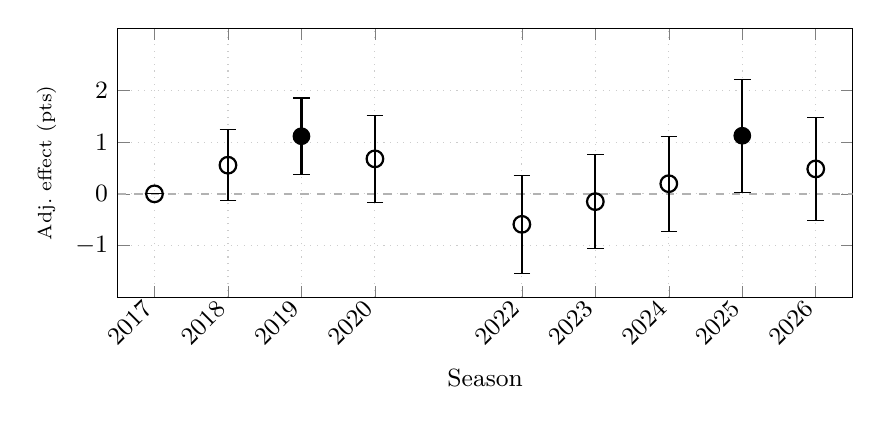
\begin{tikzpicture}
\begin{axis}[
  width=0.90\columnwidth,
  height=5.0cm,
  xlabel={Season},
  ylabel={Adj.\ effect (pts)},
  xlabel style={font=\small},
  ylabel style={font=\scriptsize},
  tick label style={font=\small},
  xmin=2016.5, xmax=2026.5,
  xtick={2017,2018,2019,2020,2022,2023,2024,2025,2026},
  xticklabels={2017,2018,2019,2020,2022,2023,2024,2025,2026},
  x tick label style={rotate=45, anchor=east, font=\small},
  ymin=-2.0, ymax=3.2,
  ytick={-1,0,1,2},
  grid=major,
  grid style={dotted, gray!40},
]
% Reference line at zero
\draw[dashed, gray!60, thick] (axis cs:2016.5,0) -- (axis cs:2026.5,0);

% Non-significant seasons (open circles with 95% CI bars)
\addplot[
  only marks,
  mark=o,
  mark size=3pt,
  mark options={fill=white, draw=black, line width=0.8pt},
  error bars/.cd,
    y dir=both, y explicit,
    error bar style={black, line width=0.8pt},
] coordinates {
  (2017, 0.0000) +- (0, 0.0000)
  (2018, 0.5536) +- (0, 0.6866)
  (2020, 0.6762) +- (0, 0.8451)
  (2022,-0.5883) +- (0, 0.9502)
  (2023,-0.1502) +- (0, 0.9116)
  (2024, 0.1965) +- (0, 0.9171)
  (2026, 0.4819) +- (0, 0.9911)
};

% Significant seasons (filled circles with 95% CI bars)
\addplot[
  only marks,
  mark=*,
  mark size=3pt,
  mark options={fill=black, draw=black},
  error bars/.cd,
    y dir=both, y explicit,
    error bar style={black, line width=0.8pt},
] coordinates {
  (2019, 1.1134) +- (0, 0.7393)
  (2025, 1.1229) +- (0, 1.0901)
};
\end{axis}
\end{tikzpicture}
\caption{Adjusted season score effects relative to 2017, controlling for class, competition week, event stage, and ensemble. Error bars show 95\% confidence intervals (standard errors clustered by ensemble). Filled markers indicate $p<0.05$: 2019 ($+1.11$ pts) and 2025 ($+1.12$ pts) are statistically higher than 2017; all other seasons are indistinguishable.}
\Description{Point and error-bar chart of adjusted season effects relative to 2017. The estimates for 2019 and 2025 are above zero with filled markers; other confidence intervals overlap zero.}
\label{fig:season-effects}
\end{figure}

